\section{Εκπαιδευόμενο Πεδίο Προσημασμένης Απόστασης - Neural SDF}
\label{section:sdf}
Στο σημείο αυτό ορίζονται κάποιες βασικές έννοιες γύρω από τοπολογικούς χώρους.  Ορίζονται, επίσης, οι βασικές δομές των συναρτήσεων οι οποίες μετρούν τα όρια των γεωμετρικών αποστάσεων με τις έμμεσες επιφάνειες.

\begin{definition}[Συνάρτηση Προσημασμένης Απόστασης]
    Αν $\Omega$ είναι ένα υποσύνολο ενός μετρικού χώρου $X$ με μετρική $d$, τότε η συνάρτηση προσημασμένης απόστασης $f$ ορίζεται ως εξής
    $$
    f(x)= \begin{cases}d(x, \partial \Omega) & \text { if } x \in \Omega \\\ -d(x, \partial \Omega) & \text { if } x \in \Omega^c\end{cases}
    $$
    όπου $\partial \Omega$ δηλώνει το όριο του $\Omega$. Για κάθε $x \in X$,
    $$
    d(x, \partial \Omega):=\inf _{y \in \partial \Omega} d(x, y)
    $$
    όπου inf δηλώνει το μέγιστο κάτω φράγμα ((\enit{infimum}). 
    Βασική συνθήκη στην οποία υπακούν συγκεκριμένα τα πεδία απόστασης με πρόσημο είναι η εικονική εξίσωση (\enit{eikonal equation}). Στην περίπτωση των πεδίων με των οποίων ασχολούμαστε αντιστοιχεί στο ότι ορίζεται για τα σημεία του χώρου που ισχύει 
    $$ |\nabla F| - 1 = 0$$, κάτι το οποίο αποτελεί πόρισμα της εξίσωσης στον ορισμό 2 που δίνεται παρακάτω \ref{eq:signeddistancefunction}
\end{definition}
\begin{definition}[Ομοιομορφισμοί]
    Οι Ομοιομορφισμοί είναι απεικονίσεις που διατηρούν τις αποστάσεις. Αν το $\boldsymbol{I}$ είναι ισομετρία (πολλαπλότητα), η απόσταση που επιστρέφεται από τον $f$ δεν χρειάζεται προσαρμογή και είναι πλήρως αντιστρέψιμος.
    $$
    d\left(\boldsymbol{x}, \boldsymbol{I} \circ f^{-1}(0)\right)=d\left(\boldsymbol{I}^{-1}(\boldsymbol{x}), f^{-1}(0)\right) .
    $$
    Οι ομοιομορφισμοί περιλαμβάνουν περιστροφές, μετατοπίσεις και ανακλάσεις.
\end{definition}
\begin{corollary} 
    Μπορούμε να θεωρήσουμε ένα ομοιομορφισμό, ως συνεχή απεικόνιση σε έκταση και κάμψη μιας τοπολογίας με τρόπο ώστε να μετα(παρα)μορφώνεται σ' ένα νέο σχήμα μέσω αυτού.
    Παράδειγμα μια κούπα καφέ και ένα ντόνατ είναι ομοιομορφικά το ένα σε σχέση με το άλλο, επειδή η κούπα μπορεί, με συνεχή παραμόρφωση, να μεταμορφωθεί σε ντόνατ (τόρο) και το αντίστροφο.
    \begin{figure}[H]
      \centering
      \begin{subfigure}{0.2\textwidth}
        \centering
        
\includegraphics[width=0.5\linewidth]{images/chapter2_img/cup.jpg}
      \end{subfigure}
      \begin{subfigure}{0.2\textwidth}
        
\includegraphics[width=0.5\linewidth]{images/chapter2_img/mid-tor-don.jpg}
      \end{subfigure}
      \begin{subfigure}{0.2\textwidth}
        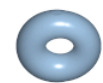
\includegraphics[width=0.5\linewidth]{images/chapter2_img/don.jpg}
      \end{subfigure}
      \caption{Ομοιομορφισμός}
    \end{figure}
\end{corollary}
\subsection{Επιφάνειες που ορίζονται από πεδία Απόστασης}
    Υπό μαθηματικούς όρους η συνάρτηση προσημασμένης απόστασης είναι ουσιαστικά μια συνάρτηση που περιγράφει την ορθογώνια απόσταση ενός δεδομένου στοιχείου \(\chi\) από το όριο ενός συνόλου \(\Omega\) σε έναν μετρικό χώρο. Αυτή η συνάρτηση, ή πεδίο, εφόσον η είσοδος και η έξοδος είναι ίσης διάστασης, μπορεί να περιγράψει κάλλιστα μια επιφάνεια Ω η οποία αναπαριστά ένα μοντέλο του φυσικού χώρου. Συνεπώς όταν αυτός ο χώρος είναι άγνωστος, εφόσον μπορούμε να ελέγξουμε τις παραμέτρους της συνάρτησης μπορούμε να ορίσουμε ποιον χώρο ακριβώς περιγράφει και η διαδικασία αυτή μπορεί να γίνει προσεγγιστικά σε νευρωνικά επίπεδα που καταγράφουν την γεωμετρία και την εμφάνιση της επιφάνειας αυτής στις παραμέτρους τους. Αυτά οδηγούνται σε μηδενική τιμή όταν αυτή η προσημασμένη απόσταση μηδενίζεται και τότε αναπαριστούν την επιθυμητή επιφάνεια. Πιο συγκεκριμένα, ο έλεγχος ενός συνόλου νευρωνικών επιπέδων που αποτυπώνει μια γεωμετρία είναι το πεδίο που εν τέλει οδηγεί στην ανακατασκευή άγνωστων επιφανειών. \\
    Συνεπώς πιο δόκιμοι ορισμοί σύμφωνα με \cite{JohnHartSphereTracing}: 
    \begin{definition}[Manifold]
        Έστω συνάρτηση \(\mathcal{F}\), με \(\mathcal{F}:\mathbb{R}^{n} \rightarrow \mathbb{R}\)  αυτή περιγράφει πολλαπλότητες, ένα σύνολο δεδομένων που αντιστοιχεί σε ισοδυναμικές επιφάνειες και μοιάζει με ευκλείδειο χώρο \(\mathcal{A}\subset{\mathbb{R}^{n}}\) ως τον γεωμετρικό τόπο των σημείων όπου: 
        \[
        \mathcal{A} = \{x : \mathcal{F}(x) \leq 0 \}
        \]
    \end{definition}

    \begin{definition}[Manifold as a Signed Distance Field]
     Μια συνάρτηση $f: \mathbb{R}^3 \rightarrow \mathbb{R}$ είναι ένα όριο απόστασης της έμμεσης επιφάνειάς της $f^{-1}(0)$ αν και μόνο αν
    \begin{equation}
        |f(\boldsymbol{x})| \leq d\left(\boldsymbol{x}, f^{-1}(0)\right),
        \label{eq:signeddistancefunction}
    \end{equation}
    
    Εάν ισχύει η ισότητα για την \ref{eq:signeddistancefunction}, τότε η $f$ είναι μια συνάρτηση απόστασης με πρόσημο. \cite{JohnHartSphereTracing}
    \end{definition}

    
    Ορισμένα πρωταρχικά στοιχεία γραφικών, όπως η σφαίρα, ορίζονται εύκολα με προσημασμένες συναρτήσεις απόστασης. Η εύρεση της απόστασης σε άλλα σχήματα μπορεί να είναι αρκετά δύσκολη. Εκεί υπεισέρχονται τα τεχνητά νευρωνικά δίκτυα προσεγγίζοντας την συνάρτηση προσημασμένης απόστασης με παλινδρομική διαδικασία. Το γεγονός ότι μπορούμε να βαδίσουμε πάνω σε μια ακτίνα με αποτέλεσμα να φτάσουμε είτε πάνω στην επιφάνεια, είτε εντός, είτε εκτός, σε συνδυασμό με το πεδίο προσημασμένης απόστασης να δίνει μηδέν στην έξοδο είτε εκτός με θετική απόσταση είτε εντός με αρνητική απόσταση ανάγει το πρόβλημα σε ένα πρόβλημα παλινδρόμησης για την εκπαίδευση παραμέτρων που αναπαριστούν άλλες γεωμετρίες.
            
\begin{figure}[H]
    \centering
    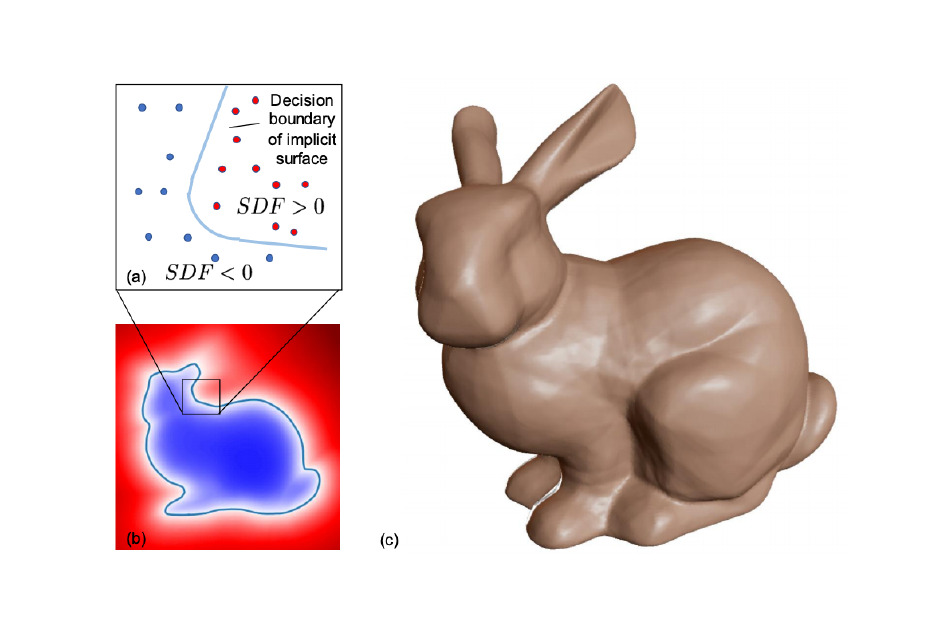
\includegraphics[width=6cm]{images/chapter2_img/DeepSDFFields.jpg}
    \caption{Ορισμός \enit{SDF} πεδίου. Πηγή \cite{yariv2020multiview}}
    \label{fig:DeepSDFlioryariv}
\end{figure}
\subsection{Διαφορίσιμες πολλαπλότητες και Γενικευμένο Θεώρημα Αναπαράστασης}

\subsubsection*{Αναπαράσταση \enit{3D} επιφάνειας μέσω νευρωνικού δικτύου}

\begin{theorem}[ θεώρημα \enit{Bocher} ή θεώρημα \enit{Representer}]
     Κάθε συμπαγής, μη υποχρεωτικά φραγμένη, τμηματικά γραμμική υπερεπιφάνεια $\mathcal{M} \subset \mathbb{R}^d$ μπορεί να αναπαρασταθεί ως ένα σύνολο νευρωνικών επιπέδων(\enit{neural level set}) $\mathcal{S}$ ενός πολυστρωματικού δικτύου perceptron με ReLU(\enit{Rectified Linear Unit}) συναρτήσεις ενεργοποίησης σε κάθε στρώμα, $F: \mathbb{R}^d \rightarrow \mathbb{R}$
     \label{theorem: Bocher's Theorem} \cite{haykin2009neural} \footnote{Απόδειξη στο Παράρτημα Β K.\ref{chapter:appendix}}.
\end{theorem} 

Σε διάφορες εργασίες δίνεται η δυνατότητα ελέγχου των δικτύων που αναπαριστούν SDF συναρτήσεις, όπως για παράδειγμα στην εκμάθηση γεωμετρίας σχηματικών αναπαραστάσεων είτε χωρίς είτε με την χρήση της πληροφορίας παραγώγων (\enit{Sign Agnostic Learning Shape})\cite{atzmon2020sal, atzmon2020sald} που αποδίδουν έμμεσα τις ισομετρικές επιφάνειες. Έτσι, ενδιαφέρον είναι να δούμε πώς γίνεται η εκπαίδευση πεδίων \enit{SDF} που αναπαριστούν διάφορες γεωμετρίες.

\subsection{Θεωρία πίσω απο τον νευρωνικό έλεγχο  διαφορίσιμων πολλαπλοτήτων(\enit{neural level sets})\cite{DBLP:journals/corr/abs-1905-11911}, \cite{haykin2009neural}}
Η χρήση δικτύων που αναπαριστούν ισομετρικές επιφάνειες και ο έλεγχος τους ώστε να αναπαριστούν τις επιθυμητές ισομετρικές επιφάνειες βασίζεται στις διαφορίσιμες πολλαπλότητες και την αμφιδιαφορισιμότητα.
\begin{definition}[Αμφιδιαφόριση - Διαφορομοιομορφισμός]
    Αν $\mathcal{X},\mathcal{Y}$  ανοιχτά σύνολα στο $\mathbb{R}^{n}$, για κάποιο  $n\in \mathbb{N}$. Τότε, λέμε ότι η απεικόνιση $f: \mathcal{X} \rightarrow \mathcal{Y}$ είναι αμφιδιαφορίσιμη (διαφορο-ομοιομορφική \enit{diffeomorphism}), εάν ισχύουν οι ακόλουθες συνθήκες:
    \begin{itemize}
        \item  η $f$ είναι ομοιομορφισμός
        \item αμφότερες $f,f^{-1}$ είναι συνεχώς διαφορίσιμες απεικονίσεις.
    \end{itemize}
    Σε αυτή την περίπτωση, τα $\mathcal{X},\mathcal{Y}$ λέγονται διαφορομορφικά σύνολα ή διαφορίσιμοι ισομετρικοί χώροι το ένα προς το άλλο. Εάν οι $f,f^{-1}$ είναι αμφότερες k-φορές συνεχώς διαφορίσιμες, τότε η f απεικόνιση αποκαλείται αμφιδιαφόριση $C^{k}$.
\end{definition}
\begin{definition}[Διαφορίσιμη Ισομετρική Επιφάνεια \cite{haykin2009neural}]
    Μια $C^{k}$ διαφορίσιμη πολλαπλότητα $\mathcal{M}$ διάστασης $n$ με σύνολο
    χαρτών επικάλυψης ή άτλαντα ομοιομορφισμών  $(X_{i},Y_{i},f_{i}),  i = 1,...,L$ είναι ένα τοπολογικό σύνολο (γενικότερη μορφή από ισομετρική επιφάνεια), όπου κάθε $\mathcal{Y_{i}}$ είναι ανοικτό σύνολο στο $\mathbb{R}^{n}$ τέτοιο ώστε οι αντιστοιχίσεις επικάλυψης $f_{ji}$ να είναι όλες αμφιδιαφορίσεις $C^{k}$  
\end{definition}
\begin{corollary}[Open Mapping Theorem]
Πόρισμα αυτού του ορισμού είναι ότι για κάθε n-διάστατο σημείο που ανήκει σε διαφορίσιμη πολλαπλότητα, $x \in \mathcal{M}$, υπάρχει ένας επιτρεπτός χάρτης απεικονίσεων $\mathcal{X,Y,f}$, όπου για $x\in \mathcal{X}$ η $f$ το αντιστοιχίζει στο $\mathcal{Y}$ που αναπαριστά άλλη τοπολογία.
\end{corollary}
    
Τα σύνολα επιπέδων νευρωνικών δικτύων (\enit{Neural Level Sets}), αναπαριστούν θεμελιώδεις ιδιότητες όπως όρια αποφάσεων κατηγοριοποιητών (\enit{classifier decision boundaries}), αλλά χρησιμοποιούνται και στην μοντελοποίηση μη γραμμικών πολλαπλοτήτων όπως καμπύλες και ισομετρικές επιφάνειες. Συνεπώς, ο έλεγχος αυτών των νευρωνικών επιπέδων μπορεί να οδηγήσει σε διάφορες εφαρμογές τεχνητής νοημοσύνης όπως στην προκείμενη περίπτωση την ανακατασκευή \enit{3D} επιφανειών μέσω ελεγχόμενων ισομετρικών επιφανειών από τις παραμέτρους νευρωνικού δικτύου SDF.


Δεδομένου ενός νευρωνικού δικτύου $F(x;\theta): \mathbb{R}^d\times\mathbb{R}^m\rightarrow\mathbb{R}^l$ το $0 \in \mathbb{R}^l$  σύνολο επίπεδου του ή (ρύθμιση του στο μηδέν στο επίπεδο εξόδου του), ορίζεται από την επιφάνεια:

$$ S(\theta) = \{x  | F(x;\theta) = 0 \}$$

Έστω πως συμβολίζεται με $D_{x}$ $F(p;\theta)\in\mathbb{R}^{l \times d}$   ο πίνακας των μερικών παραγώγων της $F$ ως προς $x$. Έστω επίσης πως οι παράμετροι γεωμετρίας $\theta$ είναι σταθερές, με $F(p;\theta) = 0$ και ότι o πίνακας των μερικών παραγώγων $D$ είναι ένας πίνακας πλήρους βαθμού (κάθε γραμμή και στήλη είναι γραμμικά ανεξάρτητες), πόρισμα του γενικού θεωρήματος ασαφών συναρτήσεων υπονοεί πως η  $S_\theta$ ισομετρική επιφάνεια είναι μια πολλαπλότητα $d-l$  διάστασης στην περιοχή του $p\in S_\theta$.

Στόχος είναι, να ενσωματωθεί σε αυτή την διαφορίσιμη πολλαπλότητα που αναπαρίσταται από νευρωνικό δίκτυο ένα διαφορικό σφάλμα. 
Αυτό επιτυγχάνεται εκτελώντας την παρακάτω διαδικασία σε κάθε εποχή εκπαίδευσης. \\
\begin{itemize}
    \item i) Δειγματοληψία $n$ σημείων πάνω στην ισομετρική επιφάνεια τέτοια ώστε: $p_i \in S\theta, i \in [n]$
    \item ii) Δημιουργία του δικτύου δειγματοληψίας $p_i(\theta), i \in [n]$ κάνοντας χρήση ενός γραμμικού νευρωνικού στρώματος στο δίκτυο της έμμεσης αναπαράστασής της γεωμετρίας της ισομετρικής επιφάνειας $F(x;\theta)$  και 
    \item iii) ενσωμάτωση μιας συνάρτησης σφάλματος στο δίκτυο δειγματοληψίας το οποίο χρησιμοποιείται ως διαμεσολαβητής στην ισομετρική επιφάνεια που αναπαρίσταται έμμεσα από την $F$.
\end{itemize} 
